\section{Snapshots of the Platform}
\begin{figure}[H]
    \centering
    \begin{subfigure}{0.8\textwidth}
        \centering
        \includegraphics[width=\textwidth]{figures/hm-landing.png}
        \caption{HealthHub Landing Page}
        \label{fig:landing_page_showcase}
    \end{subfigure}
    \vspace{1em} % Vertical space between stacked subfigures
    \begin{subfigure}{0.8\textwidth}
        \centering
        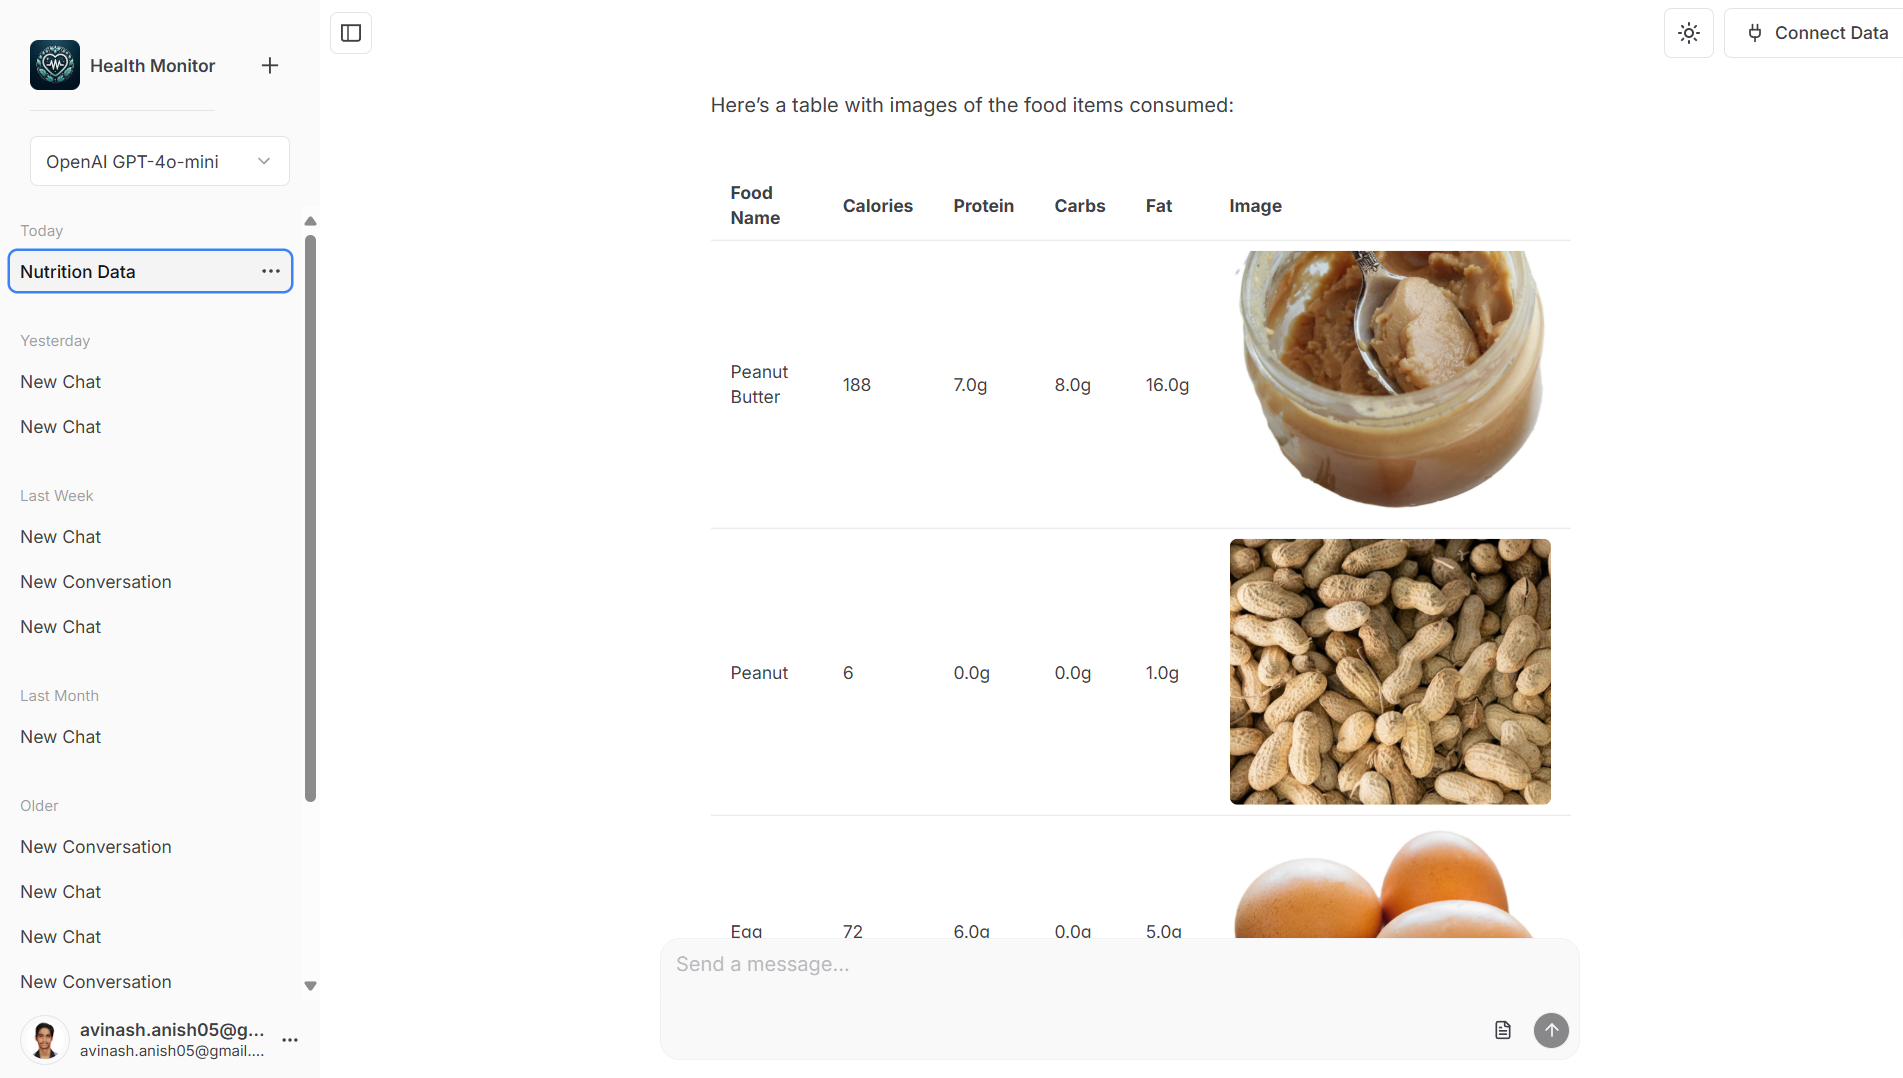
\includegraphics[width=\textwidth]{figures/hm-rag-chat.png}
        \caption{AI RAG Pipeline Chat Interface}
        \label{fig:rag_chat_showcase}
    \end{subfigure}
    \caption{Key User Interfaces: Landing Page and AI Chat}
    \label{fig:ui_showcase_pair1}
\end{figure}

\begin{figure}[H]
    \centering
    \begin{subfigure}{\textwidth}
        \centering
        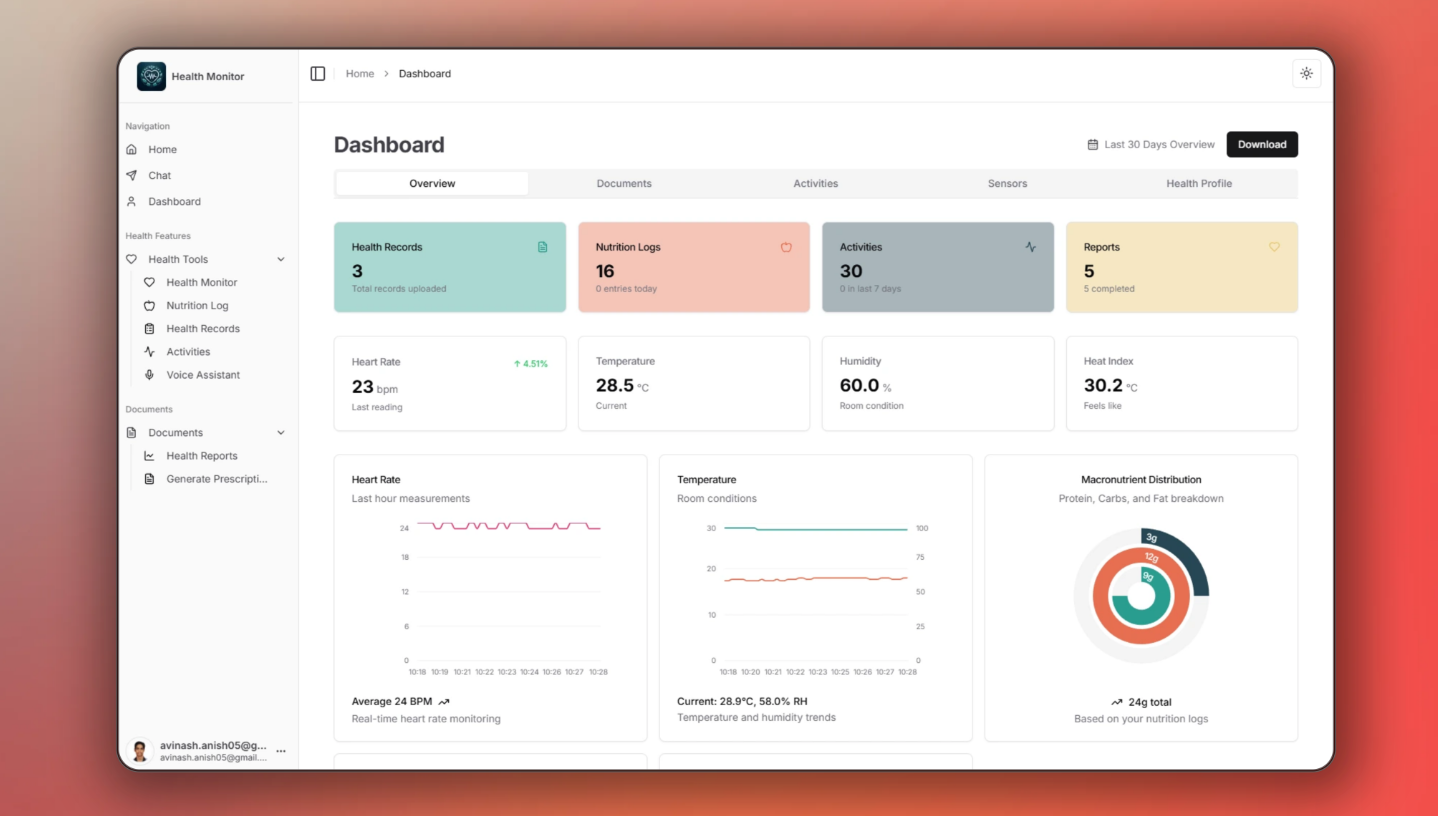
\includegraphics[width=\textwidth]{figures/hm-dashboard.png}
        \caption{Comprehensive Health Dashboard}
        \label{fig:dashboard_showcase}
    \end{subfigure}
    \vspace{1em} % Vertical space between stacked subfigures
    \begin{subfigure}{\textwidth}
        \centering
        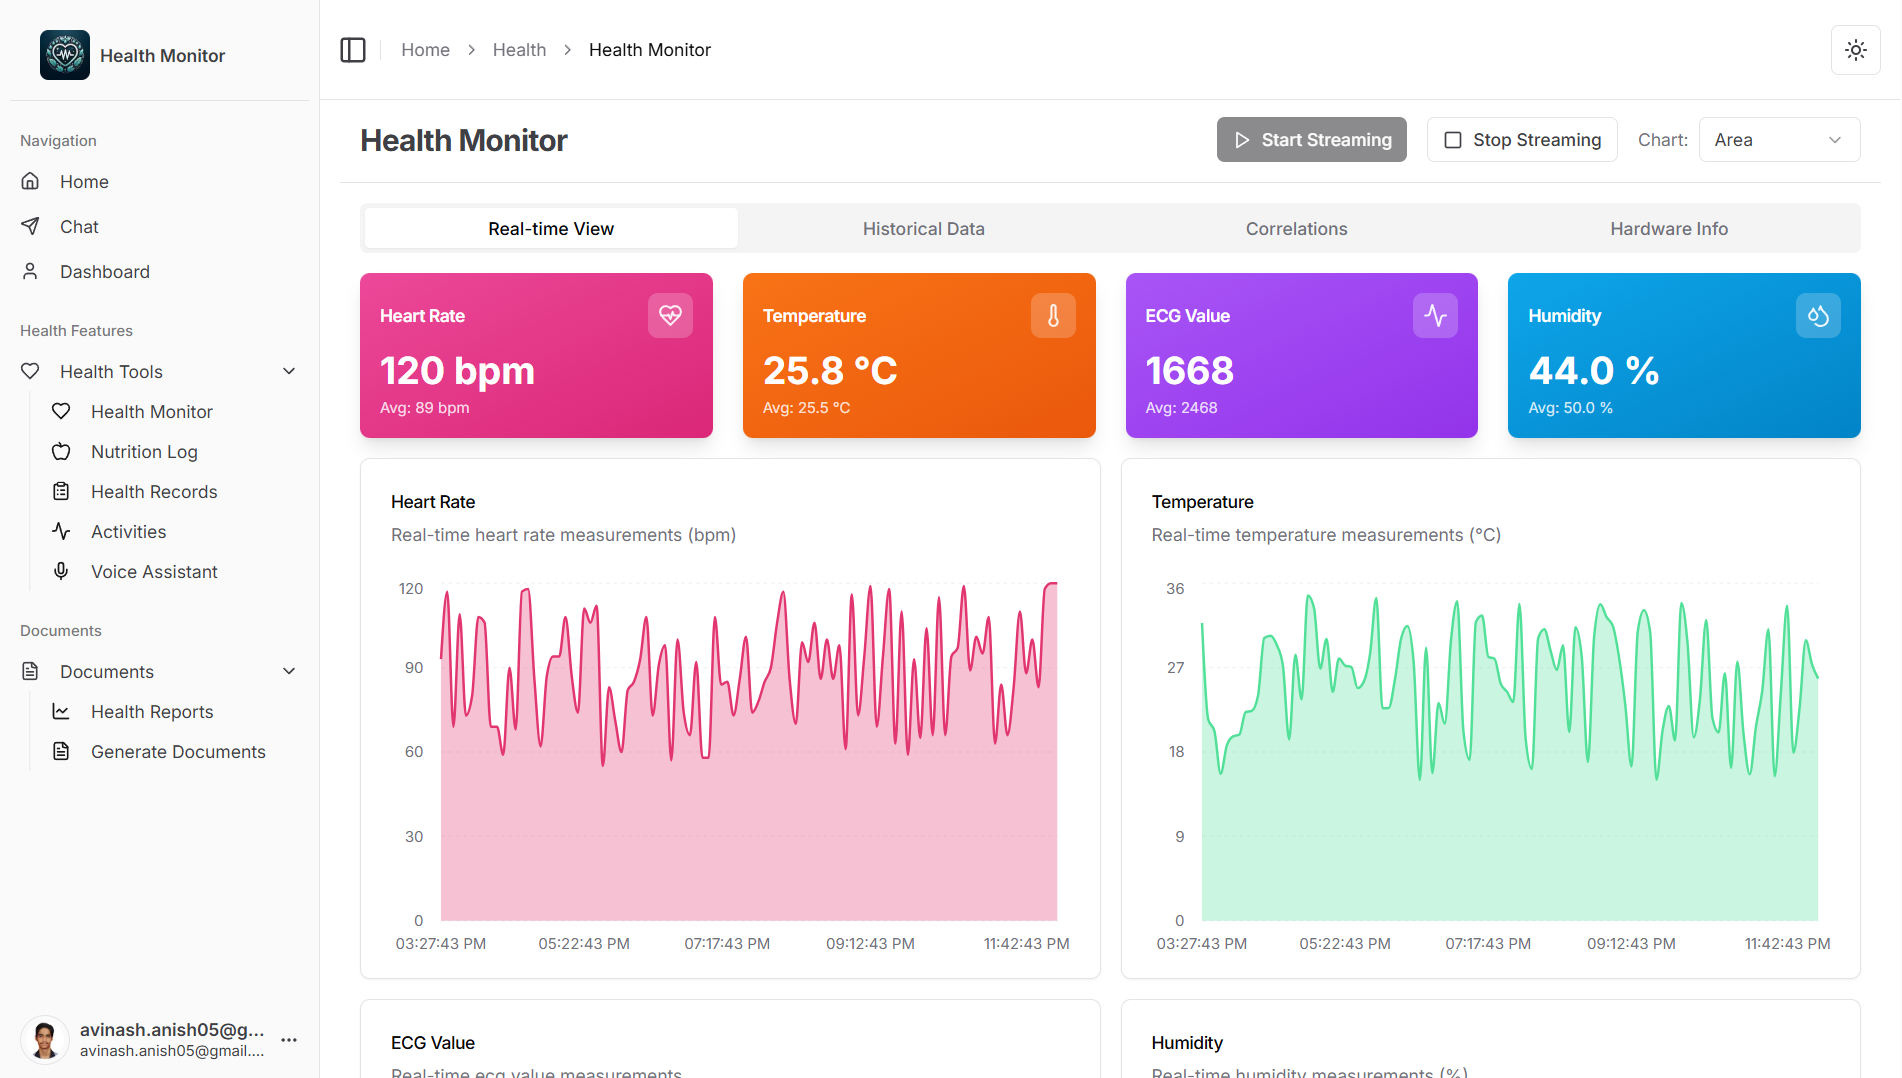
\includegraphics[width=\textwidth]{figures/hm-monitor.png}
        \caption{Real-Time Vitals Monitoring}
        \label{fig:monitor_showcase}
    \end{subfigure}
    \caption{Health Monitoring Interfaces: Dashboard and Real-Time Vitals}
    \label{fig:monitoring_showcase_pair2}
\end{figure}

\begin{figure}[H]
    \centering
    \begin{subfigure}{\textwidth}
        \centering
        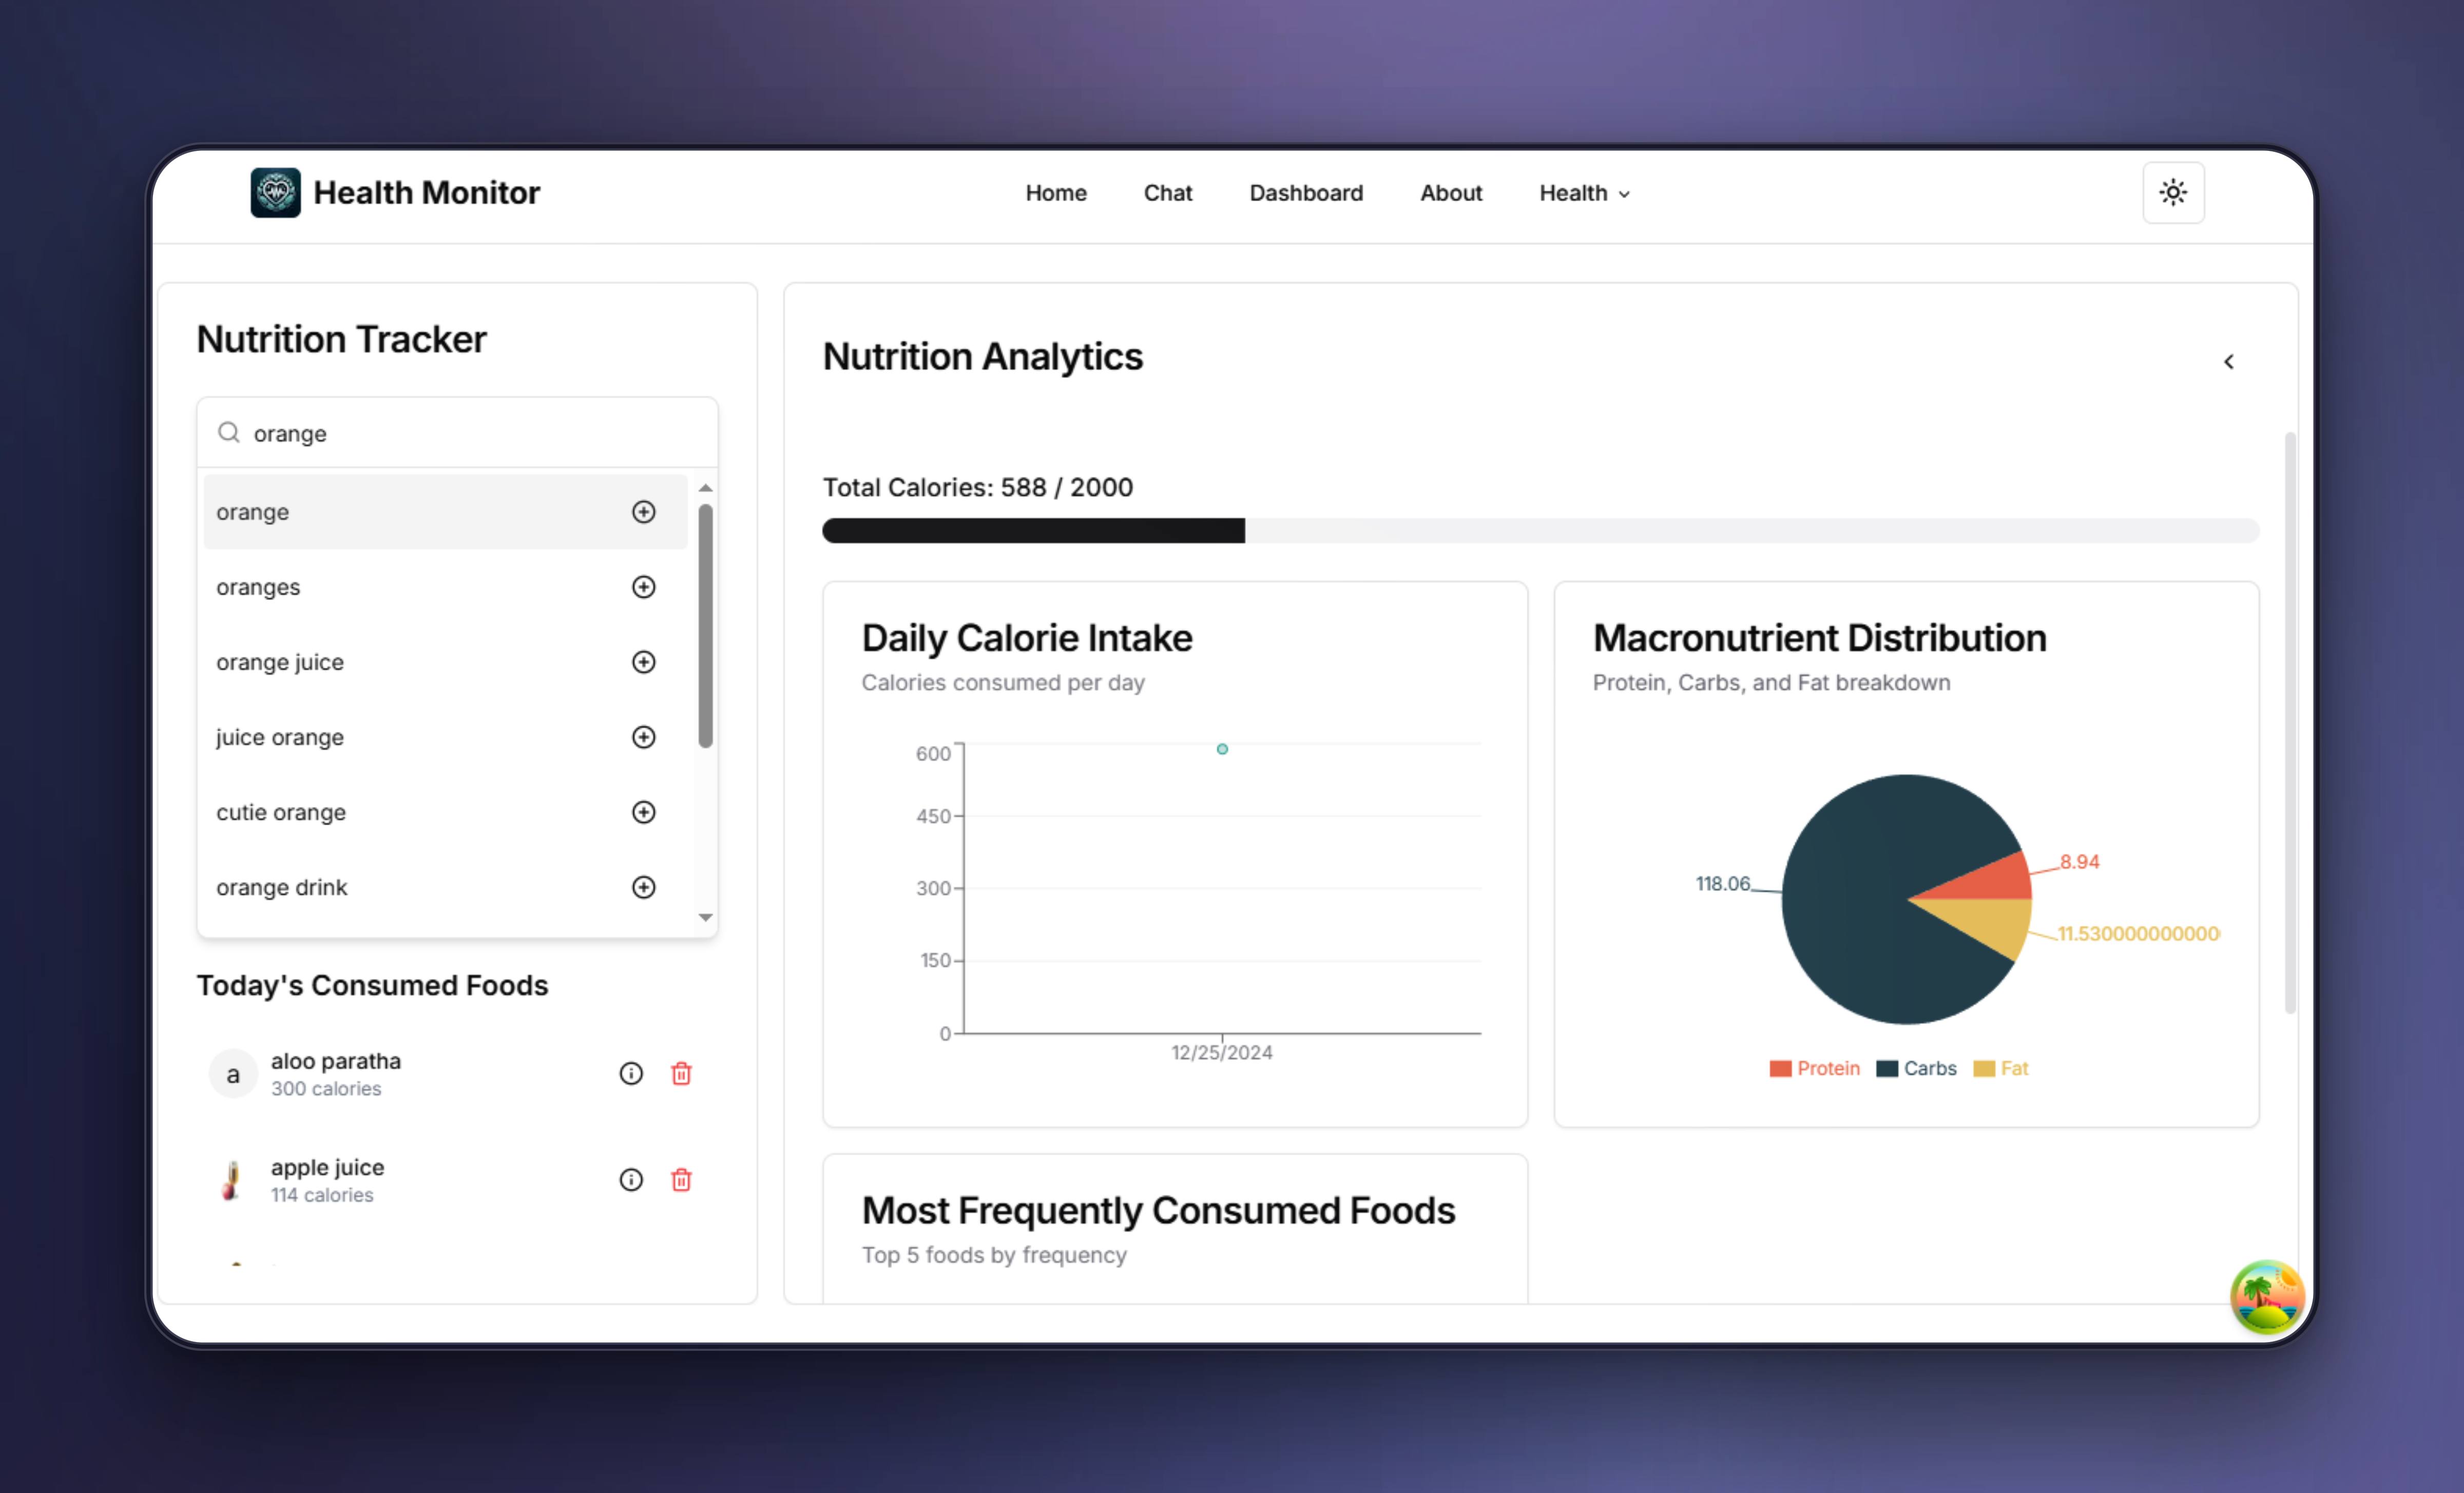
\includegraphics[width=\textwidth]{figures/hm-nutrition.png}
        \caption{Nutrition Tracking Interface}
        \label{fig:nutrition_showcase}
    \end{subfigure}
    \vspace{1em} % Vertical space between stacked subfigures
    \begin{subfigure}{\textwidth}
        \centering
        \includegraphics[width=\textwidth]{figures/hm-video-landing.png}
        \caption{Integrated Video Assistant}
        \label{fig:video_assistant_showcase}
    \end{subfigure}
    \caption{Specialized Platform Features: Nutrition and Video Assistance}
    \label{fig:specialized_features_pair3}
\end{figure}

\begin{figure}[H]
    \centering
    \begin{subfigure}{\textwidth}
        \centering
        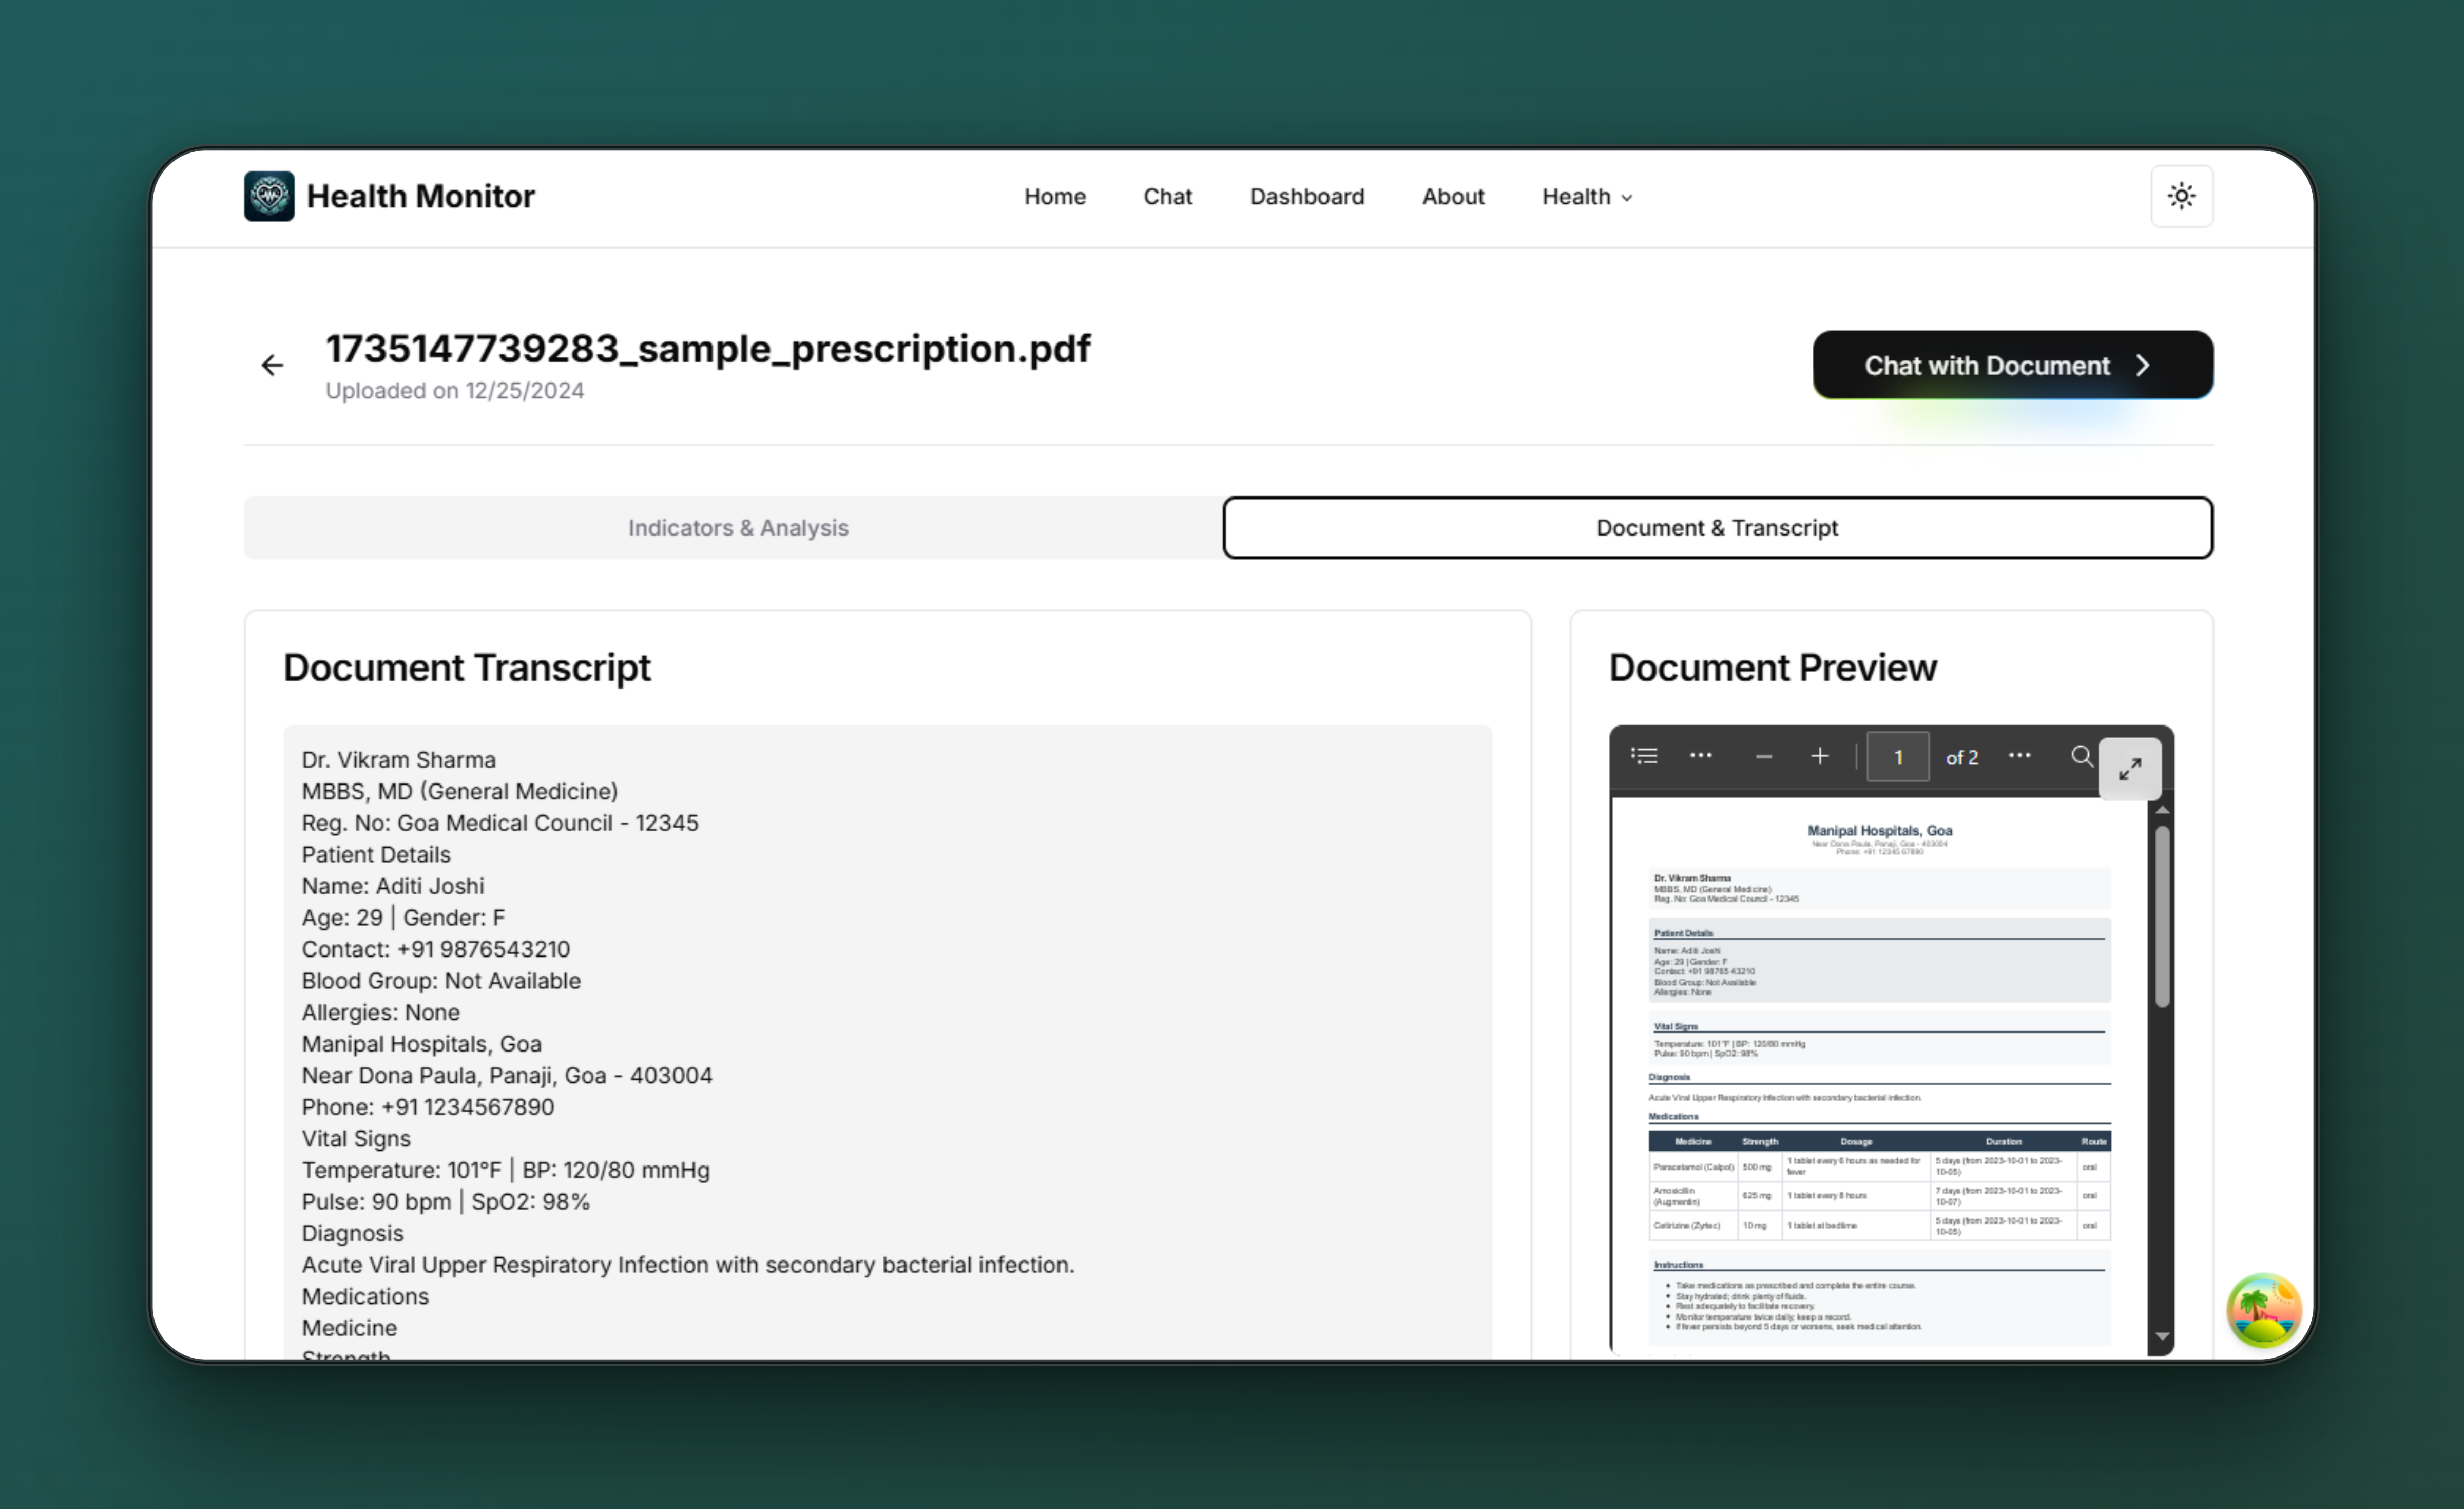
\includegraphics[width=\textwidth]{figures/hm-record-transcript.png}
        \caption{Medical Record Transcription}
        \label{fig:transcript_showcase}
    \end{subfigure}
    \vspace{1em} % Vertical space between stacked subfigures
    \begin{subfigure}{\textwidth}
        \centering
        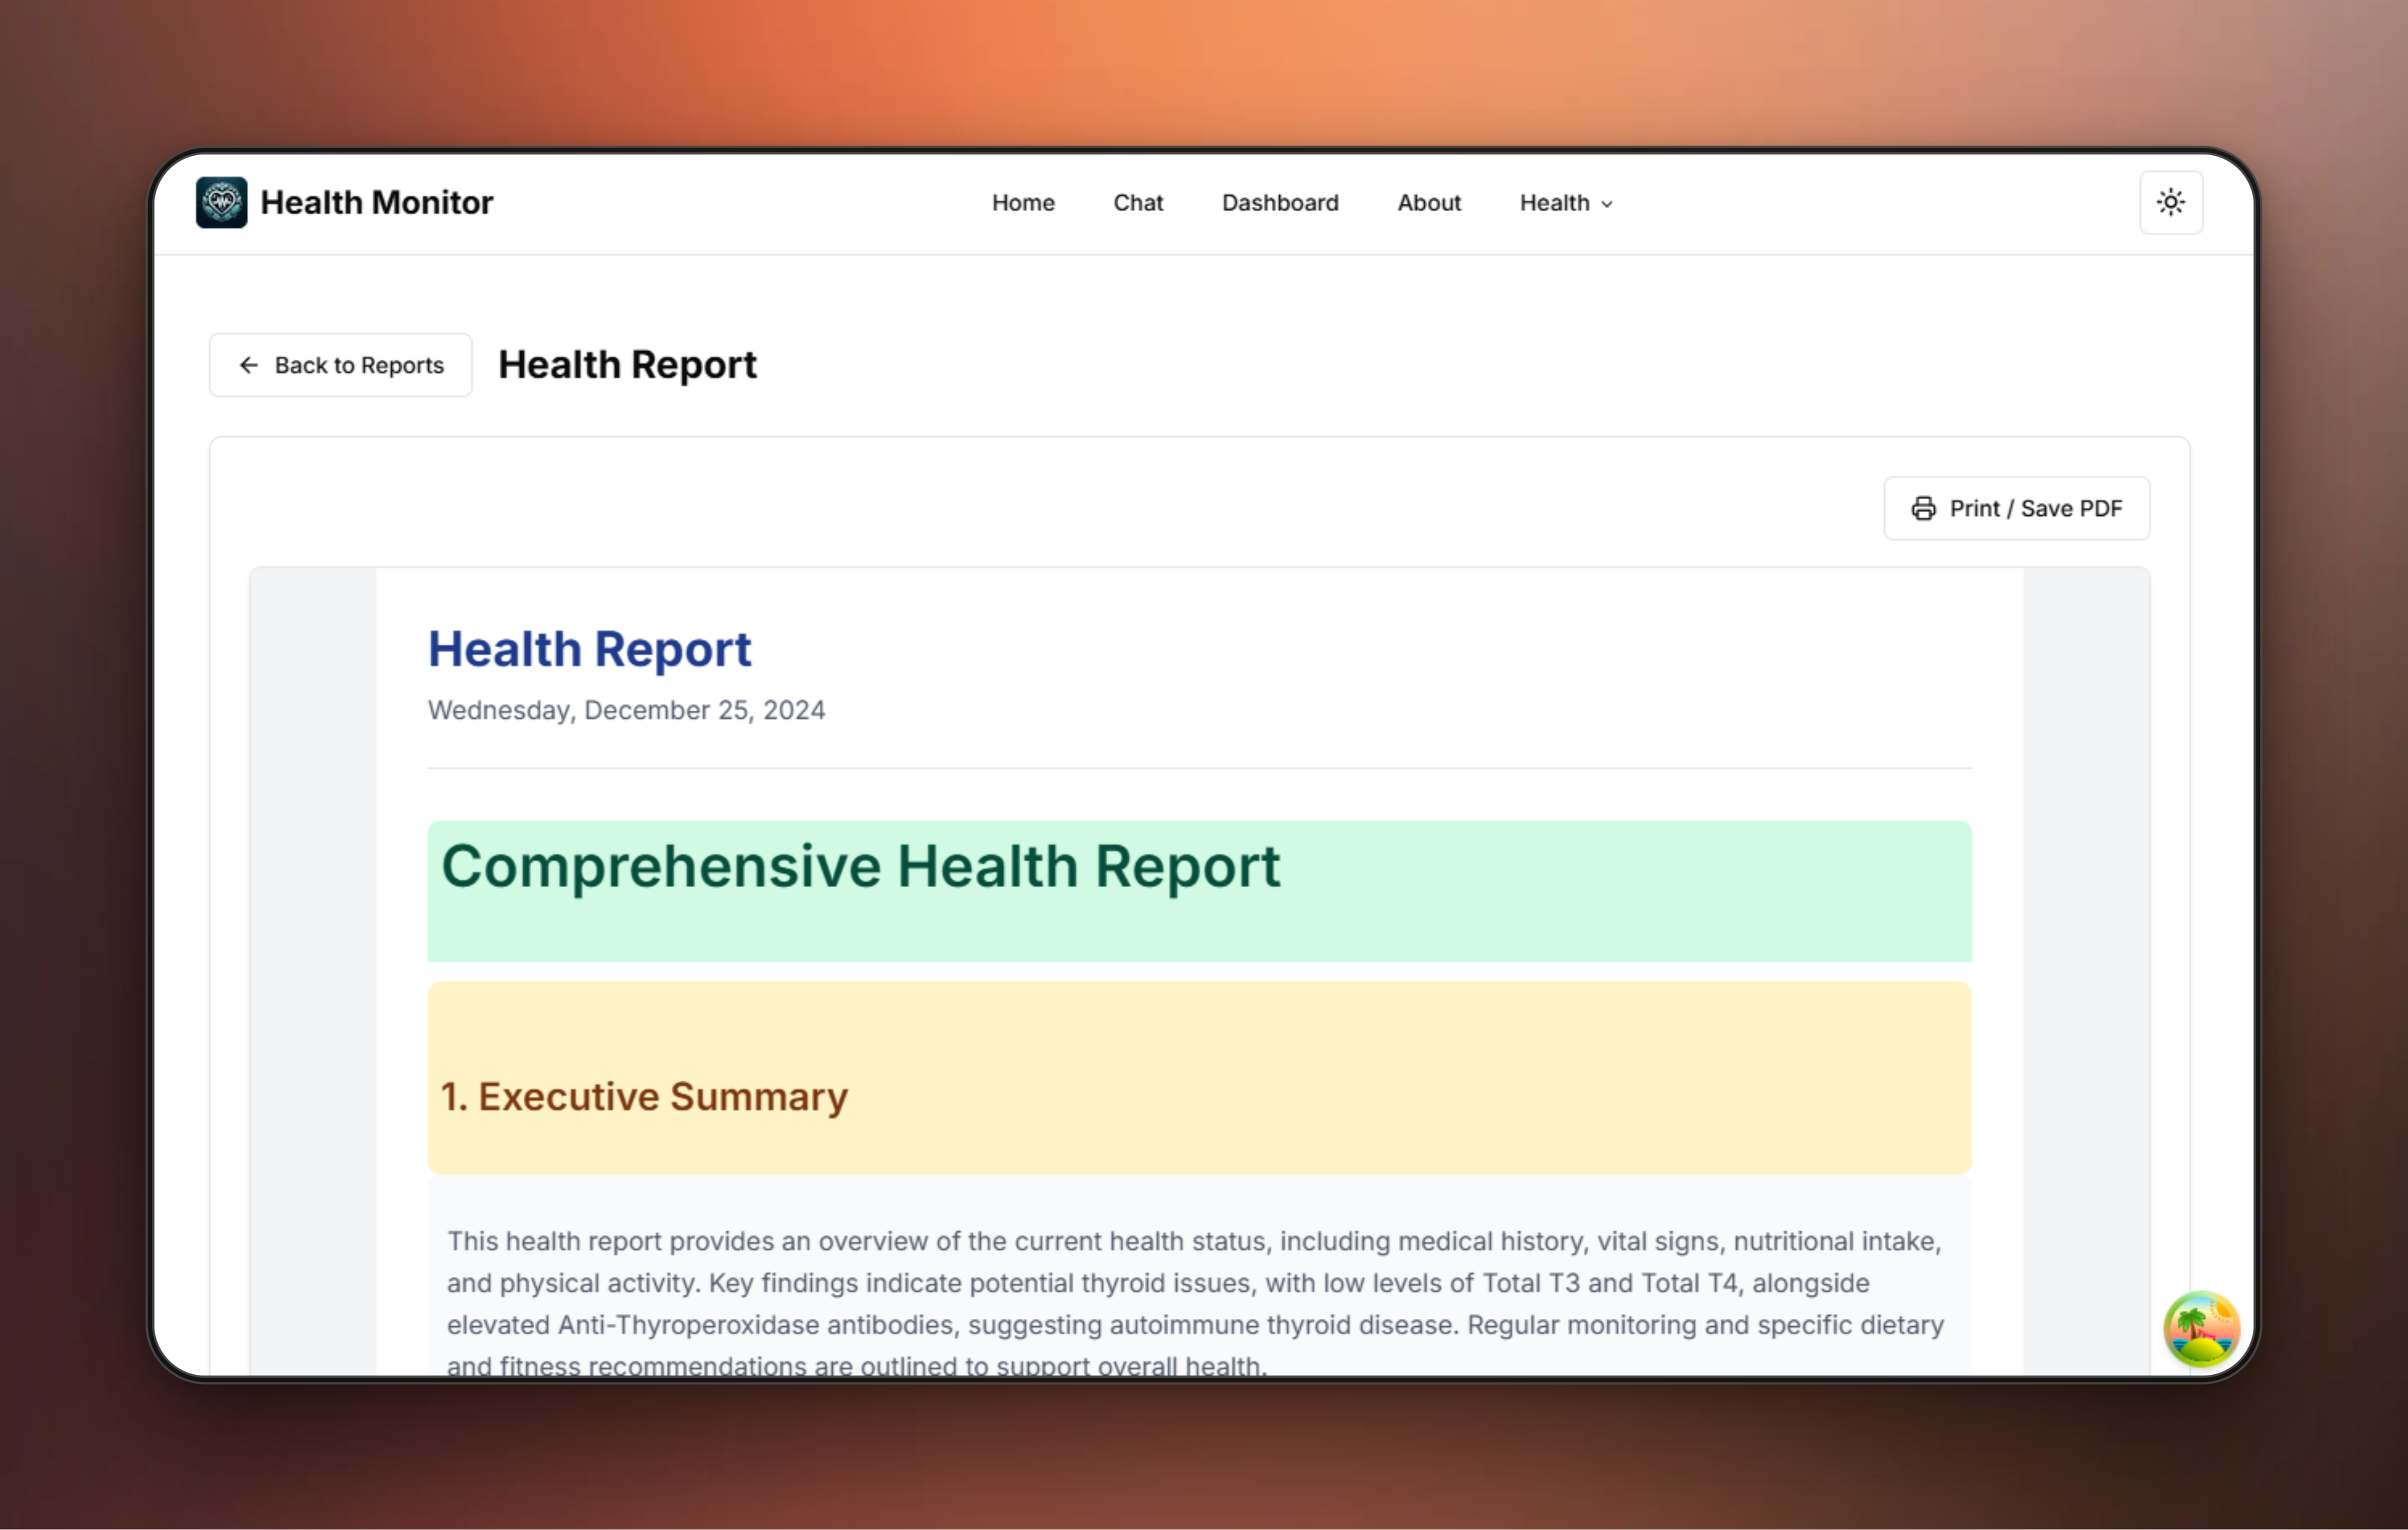
\includegraphics[width=\textwidth]{figures/hm-report.png}
        \caption{Health Report Generation}
        \label{fig:report_showcase}
    \end{subfigure}
    \caption{Automated Data Processing: Transcription and Report Generation}
    \label{fig:data_processing_pair4}
\end{figure}

\section{Execution Guide}

This section outlines the steps to set up and run the HealthHub platform, based on the project's README file.

\subsubsection*{Prerequisites}
Before starting, ensure you have the following installed and configured:
\begin{itemize}
    \item Node.js (v14 or later)
    \item Python (v3.8 or later)
    \item Arduino IDE (latest version recommended)
    \item Required Sensors: MAX30102 (Pulse Oximeter/Heart Rate), AD8232 (ECG), LM35 (Temperature), SEN-11574 (GSR)
    \item A Supabase account and project credentials
    \item API keys for: OpenAI, Gemini, Tavily, Cohere, Resend, and Nutritionix
\end{itemize}

\subsubsection*{Hardware and Firmware Setup}
This subsection details the setup for the IoT hardware components.

\paragraph*{Required Components and Software}
\begin{itemize}
    \item Arduino UNO R3 (or compatible)
    \item ESP8266 Wi-Fi Module
    \item Sensors: MAX30102 (Pulse Oximeter and Heart Rate), AD8232 (ECG), LM35 (Temperature), SEN-11574 (GSR)
    \item Breadboard and jumper wires
    \item Arduino IDE (ensure appropriate board managers and libraries are installed, e.g., MAX30100lib for MAX30102)
\end{itemize}

\paragraph*{Sensor Connections}
Connect the sensors to the Arduino UNO according to standard pin configurations or as detailed in the project's hardware documentation. Ensure all connections are secure. General guidance:
\begin{itemize}
    \item MAX30102: Typically connected via I2C (SDA, SCL pins).
    \item AD8232: Requires connections for LA, RA, RL electrodes and power.
    \item LM35: Connect to an analog input pin.
    \item SEN-11574: Connect to an analog input pin.
\end{itemize}

\paragraph*{Arduino Firmware Upload}
\begin{enumerate}
    \item Open the Arduino IDE.
    \item Navigate to the project's \texttt{arduino/} directory.
    \item Open the Arduino sketch file (e.g., \texttt{arduino\_firmware.ino}).
    \item Select "Arduino UNO" as the board and the correct port from the Tools menu.
    \item Ensure all necessary libraries for the connected sensors are installed in the Arduino IDE.
    \item Compile and upload the sketch to the Arduino UNO.
\end{enumerate}

\paragraph*{ESP8266 Firmware Upload and Configuration}
The ESP8266 module handles Wi-Fi communication.
\begin{enumerate}
    \item Ensure the ESP8266 is correctly wired for standalone operation or for programming mode (e.g., GPIO0 to GND for flashing).
    \item Open the Arduino IDE.
    \item Navigate to the project's \texttt{arduino/} directory.
    \item Open the ESP8266 sketch file (e.g., \texttt{esp8266\_firmware.ino}).
    \item Select the appropriate ESP8266 board (e.g., "NodeMCU 1.0" or "Generic ESP8266 Module") and port from the Tools menu.
    \item Ensure ESP8266 board support is installed in the Arduino IDE.
    \item Modify the sketch to include your Wi-Fi network credentials (SSID and password), as indicated within the sketch code.
    \item Compile and upload the sketch to the ESP8266 module.
    \item The ESP8266 will then connect to your Wi-Fi and communicate with the Arduino (via serial or other configured means) to relay sensor data to the backend API.
\end{enumerate}

\subsubsection*{Software Installation Steps}

\begin{enumerate}
    \item \textbf{Clone Repositories:}
    \begin{tcolorbox}[listing engine=listings, colback=black!5!white, colframe=black!75!black, title=Clone Frontend Repository, listings options={breaklines=true, basicstyle=\ttfamily\footnotesize, breakatwhitespace=true, keepspaces=true}]
git clone https://github.com/CubeStar1/health-monitor-next.git
    \end{tcolorbox}
    \begin{tcolorbox}[listing engine=listings, colback=black!5!white, colframe=black!75!black, title=Clone Backend Repository, listings options={breaklines=true, basicstyle=\ttfamily\footnotesize, breakatwhitespace=true, keepspaces=true}]
git clone https://github.com/CubeStar1/health-monitor-api.git
    \end{tcolorbox}

    \item \textbf{Install Frontend Dependencies:}
    \begin{tcolorbox}[listing engine=listings, colback=black!5!white, colframe=black!75!black, title=Install Frontend Dependencies, listings options={breaklines=true, basicstyle=\ttfamily\footnotesize, breakatwhitespace=true, keepspaces=true}]
cd health-monitor-next
npm install
    \end{tcolorbox}

    \item \textbf{Set Up Python Backend:}
    \begin{tcolorbox}[listing engine=listings, colback=black!5!white, colframe=black!75!black, title=Set Up Python Backend, listings options={breaklines=true, basicstyle=\ttfamily\footnotesize, breakatwhitespace=true, keepspaces=true}]
cd healthhub-backend  // Or path/to/health-monitor-api
python -m venv venv
# On Linux/macOS:
source venv/bin/activate
# On Windows:
# venv\Scripts\activate
pip install -r requirements.txt
    \end{tcolorbox}

    \item \textbf{Set Up Environment Variables:}
    Create \texttt{.env} files in both the frontend (\texttt{health-monitor-next}) and backend (\texttt{health-monitor-api}) root directories. Populate them with the necessary API keys and Supabase credentials as detailed in the project's README.
    
    Key variables include:
    \begin{itemize}
        \item Frontend: \texttt{NEXT\_PUBLIC\_SUPABASE\_URL}, \texttt{NEXT\_PUBLIC\_SUPABASE\_ANON\_KEY}, \texttt{NEXT\_PUBLIC\_API\_URL}, etc.
        \item Backend: \texttt{OPENAI\_API\_KEY}, \texttt{GOOGLE\_API\_KEY}, \texttt{COHERE\_API\_KEY}, \texttt{SUPABASE\_URL}, \texttt{SUPABASE\_KEY}, etc.
    \end{itemize}

    \item \textbf{Apply Database Migrations (Supabase):}
    Ensure you have the Supabase CLI installed and configured. Navigate to the backend project root (\texttt{health-monitor-api}) and run the following commands:
    \begin{tcolorbox}[listing engine=listings, colback=black!5!white, colframe=black!75!black, title=Supabase DB Migrations, listings options={breaklines=true, basicstyle=\ttfamily\footnotesize, columns=fixed, literate={<}{{\\textless}}1 {>}{{\\textgreater}}1, breakatwhitespace=true, keepspaces=true}]
# Log in to Supabase (if not already logged in)
supabase login

# Link your local project to your Supabase project
supabase link --project-ref 

# Apply migrations
supabase db push
    \end{tcolorbox}

    \item \textbf{Start Development Servers:}
    \paragraph*{Frontend Server:}
    Navigate to the \texttt{health-monitor-next} directory and run:
    \begin{tcolorbox}[listing engine=listings, colback=black!5!white, colframe=black!75!black, title=Start Frontend Server, listings options={breaklines=true, basicstyle=\ttfamily\footnotesize, breakatwhitespace=true, keepspaces=true}]
npm run dev
    \end{tcolorbox}
    \paragraph*{Backend Server:}
    Navigate to the \texttt{health-monitor-api} directory (ensure virtual environment is activated) and run:
    \begin{tcolorbox}[listing engine=listings, colback=black!5!white, colframe=black!75!black, title=Start Backend Server, listings options={breaklines=true, basicstyle=\ttfamily\footnotesize, breakatwhitespace=true, keepspaces=true}]
uvicorn main:app --reload
    \end{tcolorbox}
\end{enumerate}

For detailed instructions on medical records processing and other features, please refer to the full \texttt{README.md} in the project repositories.
